\section{Introduction}

The main goal of our project is to make a functional calculator that operates with 3 bit signed integers, in a range of [-8:7].
To input the two operands, we will use the eight switchs available on the board. The eight switches represent the eight bit word, where the 4 most significant bits represent the first operand and the other bits represent the second.

\begin{figure}[!htbp]
    \centerline{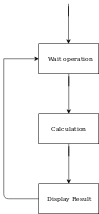
\includegraphics[width=50mm, scale=0.5]{fluxograma}}
    \vspace{0cm}\caption{Calculator flow chart}
    \label{fig:fluxograma}
\end{figure}
